\documentclass[compress,xcolor=table,aspectratio=169]{beamer}
% Packages
\usepackage{moresize} 
\usepackage[english]{babel}
\usepackage[utf8]{inputenc}
\usepackage[T1]{fontenc}
\usepackage{datetime}
\usepackage{multicol} 
\usepackage{multirow} 
\usepackage{booktabs}
\usepackage{verbatim}
%\usepackage{natbib}

% Default fixed font does not support bold face
\DeclareFixedFont{\ttb}{T1}{txtt}{bx}{n}{12} % for bold
\DeclareFixedFont{\ttm}{T1}{txtt}{m}{n}{12}  % for normal
% Custom colors
\usepackage{color}
\definecolor{deepblue}{rgb}{0,0,0.5}
\definecolor{deepred}{rgb}{0.6,0,0}
\definecolor{deepgreen}{rgb}{0,0.5,0}
\usepackage{listings}
% Python style for highlighting
\lstset{
language=Python,
basicstyle=\scriptsize\tt,
otherkeywords={self},             % Add keywords here
%keywordstyle=\ttb\color{deepblue},
%emph={MyClass,__init__},          % Custom highlighting
%emphstyle=\ttb\color{deepred},    % Custom highlighting style
stringstyle=\color{deepgreen},
frame=tb,                         % Any extra options here
showstringspaces=false            % 
}

\usepackage{graphicx}
\usepackage{epsfig}
\usepackage{amsmath}
\usepackage{amsfonts}
\usepackage{amssymb}
%\usepackage{pstricks}
\usepackage{bbold}

\def\ok{\color{green!80!black} $\mathbf +$}
\def\notok{\color{red} $\mathbf -$}

\newcommand\warning{\includegraphics[width=.7cm,keepaspectratio]{../logos/warning}}
\def\plus{\color{green!80!black} $\mathbf +$}
\def\moins{\color{red} $\mathbf -$}
\newcommand\bibref[4][1]{
\hspace*{-0.5cm}   
\begin{tabular}{m{0.6cm}m{#1\linewidth}}
    \includegraphics[width=.7cm,keepaspectratio]{../logos/book}  & 
      \scriptsize  {\color{black} \textit{#2}}, #3 \newline #4  
   \end{tabular}
   }



\def\espace{\hspace*{5mm}}

\DeclareMathOperator*{\argmin}{arg\,min}
\DeclareMathOperator*{\argmax}{arg\,max}
\DeclareMathOperator*{\Log}{Log} 
\DeclareMathOperator*{\Exp}{Exp}


\def\cov{\mbox{cov}}

\def\R{\mathbb{R}}
\def\C{\mathbb{C}}
\def\N{\mathbb{N}}
\def\Q{\mathbb{Q}}
\def\Z{\mathbb{Z}}

\def\esp{\mathbb{E}}
\def\var{\mathbb{V}}
\def\P{\mathbb{P}}


\def\mA{\mathcal{A}}
\def\mB{\mathcal{B}} 
\def\mC{\mathcal{C}}

\def\mP{\mathcal{P}}
\def\mN{\mathcal{N}}
\def\mF{\mathcal{F}}
\def\mH{\mathcal{H}}

\def\bs{\mathbf{s}}
\def\bx{\mathbf{x}}
\def\bd{\mathbf{d}}
\def\bu{\mathbf{u}}
\def\bi{\mathbf{i}}
\def\bj{\mathbf{j}}
\def\by{\mathbf{y}}



\def\bX{\mathbf{X}}
\def\by{\mathbf{y}}
\def\bY{\mathbf{Y}}
\def\bbeta{\mathbf{\beta}}
\renewcommand{\epsilon}{\varepsilon}


\def\TBE{\emph{\textsc{To be extended.}}}
\def\TBD{\emph{\textsc{To be done.}}}
\def\EOP{\emph{\textsc{End Of Proof}}}


\newcommand{\myarr}[1]{
    \begin{array}{ccccccccc} #1
    \end{array}
}
\newcommand{\matrice}[1]{
   \left[ \begin{array}{ccccccccc} #1
    \end{array}
    \right]
}
\newcommand{\TOSEE}[1]{ {\red
\begin{pspicture}(0,0)
  \rput(-2.3,0){
    \begin{minipage}[h]{2.5cm}
      #1
    \end{minipage}
}
\end{pspicture}}
}

\newcommand{\im}{\mbox{Im}}

\usepackage{float}

\newcommand{\st}{\mbox{s.t. }}
\newcommand{\tq}{\mbox{tel que }}

\floatstyle{ruled}
\newfloat{algo}{htbp}{alg}[section]
\floatname{algo}{Alg.} % titre du caption
\newcommand{\sign}{\mbox{sign}}
\newcommand{\energy}{\mathcal{E}}
\newcommand{\diag}{\mbox{diag}}

\newcommand\bw{\mathbf{w}}
%\newcommand\bx{\mathbf{x}}

\newcommand{\bbun}{\mbox{\textbb 1}}
\newcommand{\bbN}{\mathbb{N}}
\newcommand{\bbC}{\mathbb{C}}
\newcommand{\bbR}{\mathbb{R}}
\newcommand{\bbQ}{\mathbb{Q}}
\newcommand{\bbZ}{\mathbb{Z}}
\newcommand{\bbP}{\mathbb{P}}
\newcommand{\bbK}{\mathbb{K}}

\newcommand{\eme}{^{\grave{e}me}}

\newcommand{\calA}{\mathcal{A}}
\newcommand{\calB}{\mathcal{B}}
\newcommand{\calC}{\mathcal{C}}
\newcommand{\calD}{\mathcal{D}}
\newcommand{\calE}{\mathcal{E}}
\newcommand{\calF}{\mathcal{F}}
\newcommand{\calG}{\mathcal{G}}
\newcommand{\calH}{\mathcal{H}}
\newcommand{\calK}{\mathcal{K}}
\newcommand{\calL}{\mathcal{L}}
\newcommand{\calM}{\mathcal{M}}
\newcommand{\calN}{\mathcal{N}}
\newcommand{\calR}{\mathcal{R}}
\newcommand{\calS}{\mathcal{S}}
\newcommand{\calW}{\mathcal{W}}


\newcommand{\bz}{\mathbf{z}}
\newcommand{\calT}{\mathcal{T}}
\newcommand{\calX}{\mathcal{X}}
\newcommand{\calY}{\mathcal{Y}}


\newcommand{\intall}{\int_{-\infty}^{+\infty}}

\newcommand{\e}{\mbox{e}}
\newcommand{\dist}{\mbox{dist}}
\newenvironment{remarquetmp}{\\ \color{red}}{\\}
\newcommand{\ra}{\rightarrow}
\newcommand{\la}{\leftarrow}
\newcommand{\ssi}{\Longleftrightarrow}
\newcommand{\implique}{\Longrightarrow}
\newcommand{\Ra}{\Longrightarrow}
\newcommand{\card}{\mbox{card}}
\newcommand{\asin}{\mbox{asin}}
\newcommand{\acos}{\mbox{acos}}
\newcommand{\second}{{\prime\prime}}
\newcommand{\tierce}{{\prime\prime\prime}}
\newcommand{\tsp}{^{\small T}}

\newcommand{\bul}{$\bullet$ }

\newcommand{\tocheck}[1]{{\red \emph{#1}} }

\newcommand{\vect}[1]{\overrightarrow{#1}}
\newcommand{\1}{\mbox{\textbb 1}}


\newcommand{\err}{\calC} %{\mbox{err}}
%\newcommand\argmin[1]{\underset{\mbox{\footnotesize $#1$}}{\mbox{argmin}}}
\newcommand{\egint}{\overset{\scriptsize ?}{=}}

\newcommand\figwidth[2]{\includegraphics[width=#1\textwidth]{#2}}
\newcommand\figheight[2]{\includegraphics[height=#1\textwidth]{#2}}

\newcounter{Exo}[section]

\newenvironment{disarray}%
 {\everymath{\displaystyle\everymath{}}\array}%
 {\endarray}

%\makeatletter
%\newcommand{\exercice}[1]{\stepcounter{Exo} {-3.5ex \@plus -1ex \@minus -.2ex} \textbf{\large Exercice \theExo~: #1} {2.3ex \@plus.2ex}}
%\makeatother
\newcommand{\espacereponse}[1]{
\noindent
\fbox{
  \begin{minipage}{1.0\linewidth}
    \vspace*{#1}


    \hspace*{1.0\linewidth}
  \end{minipage}

}}

\newcommand{\lignehorcentre}{
\noindent
%\linethickness{2}
\begin{picture}(0,0)(0,0)
 %\psline(0mm,3mm)(15.5cm,3mm) %
  \line(1,0){450}
\end{picture}\\
}
\newcommand{\myhline}{
%\vspace*{-0.5cm}
\noindent
\begin{picture}(0,-12)(0,-12)
  \line(1,0){450}
\end{picture} 
%\vspace*{-3mm}
}


\usepackage[absolute,overlay]{textpos}
  \setlength{\TPHorizModule}{1mm}
  \setlength{\TPVertModule}{1mm}

% Possible options of the package (add/remove below in \usetheme call):
%  - nosectionpages: no pages between sections
%  - flama: use flama font, requires xelatex/lualatex + the font to compile
%  - compressminiframes: put the heading list bullets indications pages on 1 line
\usetheme[compressminiframes]{sorbonne}

\newcommand{\titlecaption}[3][]{\caption[#2]{\textbf{#2}\ifthenelse{\equal{#1}{}}{. }{ }#3}}

\title{\Large{\textbf{Deep Natural Language Processing for User Representation}}}

\subtitle{Talk at the Paris NLP Meetup} % optional subtitle
\date{\formatdate{29}{9}{2021}}

\author{Clara Gainon de Forsan de Gabriac}
\institute{LIP6 - Sorbonne Université} % Optional

\usepackage[backend=biber,style=authoryear, citestyle=authoryear]{biblatex}
\bibliography{biblio}

\begin{document}

\begin{frame}[plain]
	%\titlepage
	\setcounter{framenumber}{0}
\end{frame}  
  
 
 \begin{frame}
    \frametitle{My Ph.D. in a nutshell}
        \onslide<1->{
        \begin{center}
        \Large
        Using \textbf{Natural Language Processing} for learning \textbf{versatile} \textbf{User Representations}.
        \end{center}
}
      \begin{columns}
        \begin{column}{0.5\textwidth}

        \onslide<2->{
    \begin{block}{In the domains of:}
         \begin{itemize}
            \item Recommendation and
            \item Professional Profile Learning
        \end{itemize}
    \end{block}}
    \end{column}
        \begin{column}{0.5\textwidth}
        \onslide<3->{
            \begin{block}{Key Principles}
                \begin{itemize}
                    \item User Profiles
                    \item Representation Learning
                    \item Natural Language Processing
                \end{itemize}
            \end{block}
            }
        \end{column}
    \end{columns}

\end{frame}
  
\begin{section}{Motivations}
    \begin{frame}{Motivations}
        \begin{block}{User Representation}
              \begin{itemize}
                    \item AI for users (Recommendation, coaching\dots)
                    \item Richness of profiles
                    \item Need for Professional Profile Learning
%                    \item LinkedIn: great playground
              \end{itemize}
          \end{block}
          \begin{block}{Representation Learning}
          \begin{itemize}
                \item Trend in Deep Learning
                \item Increasing need for versatile representations
          \end{itemize}
      \end{block}
      \begin{block}{Natural Language Processing}
          \begin{itemize}
              \item User-generated texts = greatly descriptive
              \item Massive amount of available data
              \item Text Generation = explainability
          \end{itemize}
      \end{block}
    \end{frame}
\end{section}

\begin{section}{Approach}
    \begin{frame}{NLP for User Representation}
        \onslide<1->{
            \begin{block}{Recommendation}
                \begin{itemize}
                    \item Reviews + ratings  $\rightarrow$ prediction accuracy
                    \item Attention Mechanism  $\rightarrow$ Explainability
                \end{itemize}
            \end{block}
            }
        \onslide<2->{
            \begin{block}{Professional Profile Learning}
                \begin{itemize}
                    \item User-generated text $\rightarrow$ build their representation
                    \item Reminder of the profile $\rightarrow$ evaluation
                \end{itemize}
            \end{block}
            }
    \end{frame}
    
\end{section}

\begin{frame}{Outline}
    \setbeamertemplate{section in toc}[circle]  
    \tableofcontents[currentsubsection, 
    hideothersubsections, 
    sectionstyle=show, 
    subsectionstyle=show]
\end{frame}


\begin{section}[Refining UR with NLP]{Refining User Representation with NLP}
\begin{frame}{Refining User Understanding in Recommendation via NLP}
\begin{columns}
  \begin{column}{.35\textwidth}
  \onslide<1->{
  \begin{block}{\centering  Intuition}
    \centering  Reviews can help improve recommendation performances \& make predictions understandable.
    \end{block}
    }
     \onslide<2->{
    \begin{block}{\centering Approach}
    \begin{center}
        Traditional rating regression \\
    +\\
    attentive sentiment analysis
    \end{center}
    \end{block}
    }
  \end{column}
    \begin{column}{.65\textwidth}
     \onslide<2->{
        \begin{figure}
            \centering
            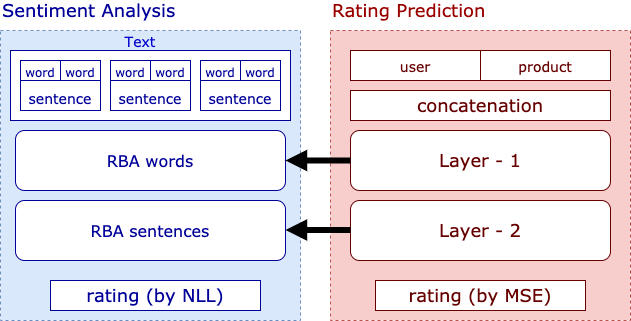
\includegraphics[width=\textwidth]{img/coriaModel.png}
            \caption{General view of the Hierarchical Recurrent Attentive Network (HRAN).}
             \label{fig:coriaOverview}
        \end{figure}
        }
  \end{column}
\end{columns}
    
\end{frame}

\begin{frame}{Model - RBA}
    \begin{figure}
        \centering
        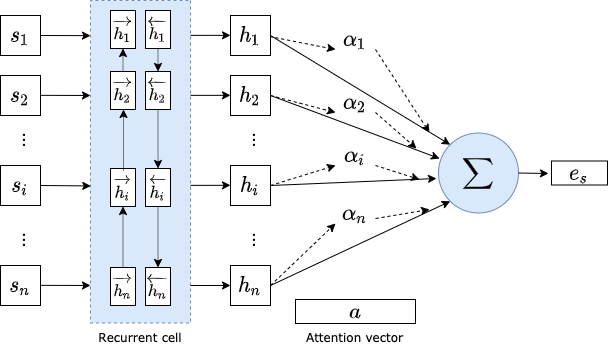
\includegraphics[height=.7\textheight]{img/RBA.png}
        \caption{Recurrent Bi-directional Attention Module, based on the work of \cite{yang2016hierarchical}.}
        \label{fig:coriaOverview}
    \end{figure}
\end{frame}

\begin{frame}{Model - Details}
    \begin{figure}
        \centering
        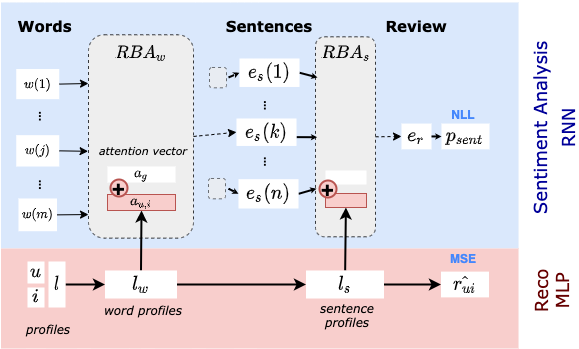
\includegraphics[height=.8\textheight]{img/globalArchOverviewCoria.png}
        \caption{ \centering Detailed view of the model for an input of $n$ sentences of $m$ words.}
        \label{fig:coriaOverview}
    \end{figure}
\end{frame}

\begin{frame}{Results - RMSE}
    \begin{table}[t]
    \centering
    \begin{tabular}{@{}llllll@{}}
    \toprule
    Dataset  (\#reviews)        & Mean $(\mu)$  & w/offset & FM 	& TransNet & HRAN  \\ \midrule
    Instant Video  (37.126)     & 1.25 			&  1.137   &    1.024   & 1.526 	&\textbf{0.937} \\
    Digital Music (64,706)      & 1.19	 		&   0.965  &    0.903 	& 1.522 	& \textbf{0.838}  \\
    Video Games  (231,780)      & 1.45	 		&   1.281  & 	1.267  	& 1.313  	&  \textbf{1.076} \\
    CSJ (278,677)               & 1.215 		&   1.323  &    1.365	& 1.285 	&  \textbf{1.081} \\
    Movie (1,697,533)           & 1.436	 		&   1.148  &    1.118 	& 1.359  	& \textbf{1.058} \\
    \bottomrule
    \end{tabular}
    \titlecaption{\centering RMSE in rating prediction}{} \label{tab:recoRMSE}
\end{table}
\end{frame}
% \begin{frame}{Results, Sentiment Analysis}
%     \begin{table}[t]
    \centering
    \begin{tabular}{@{}lllll@{}}
    \toprule
                        & FastText  &  HAN  & NSUPA  & HRAN         \\ \midrule
    Instant Video       & 62.60        & 64.50 &   65.88   & \textbf{66.60}          \\
    Digital Music       & 63.58        &   68.03   &   \textbf{70.08}   & 68.80          \\
    Video Games         & 62.51       &   67.67  &   68.60   & \textbf{69.11}            \\
    CSJ	                & 67.83        &    71.96  &   \textbf{71.99}   & 71.49          \\
    Movies              & 64.56       &   68.95   	&   71.20   & \textbf{71.62 }           \\\bottomrule
    \end{tabular}
    \titlecaption{\centering Accuracy metric on the sentiment analysis task}{}\label{tab:sentacc} 
    \end{table}
% \end{frame}

\begin{frame}{Attention Visualization}
    \begin{figure}[t]
    \begin{minipage}[c]{.48\linewidth}
        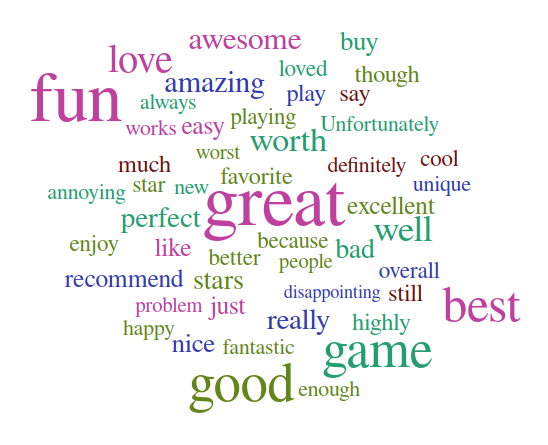
\includegraphics[width=\linewidth]{img/adj.png}
    \end{minipage} \hfill
    \begin{minipage}[c]{.48\linewidth}
        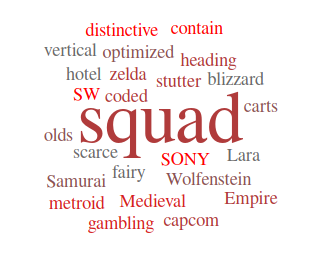
\includegraphics[width=\linewidth]{img/new_words2.png}
    \end{minipage}
    \titlecaption{ \centering  Word clouds}{Obtained by retrieving the attention scores of both modules.}
    \label{fig:att_adj_atr}
\end{figure}

\end{frame}
    \begin{frame}{Conclusion}
        \begin{itemize}
            \item Leveraging textual reviews $\rightarrow$ better performances
            \item Multi-task-learning $\rightarrow$ better performances
            \item The Attention mechanism $\rightarrow$ explainable predictions
        \end{itemize}
    \end{frame}
\end{section}

\begin{section}[PPL]{Professional Profile Learning}
\begin{frame}{Professional Profile Learning}
\onslide<1->{
    \begin{block}{\centering Problem}
    \centering 
    People tend to change jobs more and more often.\\
    How do we match job offers to candidates?
    \end{block}
    }
    \onslide<2->{
    \begin{block}{Intuition}
    \begin{itemize}
        \item We can use their LinkedIn page to build their professional profiles.
        \item Their past jobs (natural language) should be enough to represent them.
    \end{itemize}
    \end{block}
    }
\end{frame}


\begin{frame}{Professional Profile Learning - Approach}
    \begin{columns}
        \begin{column}{.5\textwidth}
        \onslide<1->{
    \begin{block}{Approach}
        \begin{itemize}
            \item User-generated text $\rightarrow$ build their representation
            \item Reminder of the profile $\rightarrow$ evaluation
        \end{itemize}
    \end{block}
    }
        \end{column}
        \begin{column}{.5\textwidth}
        \onslide<2->{
                \begin{figure}
                \centering
                \includegraphics[height=.75\textheight]{img/user.pdf}
                \caption{A LinkedIn's profile schema.}
                \label{fig:user}
              \end{figure}
              }
        \end{column}
    \end{columns}
\end{frame}

% \begin{frame}{LinkedIn Profile}
% \begin{figure}[ht]
%     \centering
%     \includegraphics[width=\textwidth]{img/userSchema.pdf}
%     \titlecaption{A LinkedIn user profile schema}
%     {}
%     \label{fig:userSchema}
% \end{figure}
% \end{frame}
    \begin{frame}{Resumé Framework}
        \begin{figure}
            \centering
            \includegraphics[height=.8 \textheight]{img/modelOverview.pdf}
            \titlecaption{A schematic representation of our architecture}{}
            \label{fig:modelOverview}
        \end{figure}
    \end{frame}
    
    \begin{frame}{Data Facts}
        \begin{columns}
            \begin{column}{.3\textwidth}
                \begin{center}
    \begin{table}[ht]
    \centering
    \begin{tabular}{@{}ll@{}}
    \multicolumn{2}{c}{Global Dataset Information} \\ \hline
    Total Profiles       & 740,983                 \\
    Train Split          & 445,097       \\
    Valid Split          & 147,909       \\
    Test Split           & 147,977   \\ \# Skills               & 523                     \\
    \# Industries            & 150                    
    \end{tabular}
    \titlecaption{\centering General dataset information}{}
    \end{table}\label{tab:geninfo}
\end{center}
            \end{column}
            \begin{column}{.7\textwidth}
                \begin{table}[ht]
    \centering
    \begin{tabular}{@{}ccccc@{}}
    %\cmidrule(l){2-5}
    \multirow{2}{*}{} & \multicolumn{2}{c}{\# exp. per profile} & \multicolumn{2}{c}{Exp. seq. len.} \\
                      &  \small Professional               &   \small Education               &   \small Professional            &   \small Education            \\ \midrule
    Average           & 5.8                        & 2.4                     & 47.5                    & 10.7                 \\
    Median            & 5                          & 2                       & 34                      & 10                   \\
    Min               & 3                          & 1                       & 5                       & 5                    \\
    Max               & 8                          & 4                       & 64                      & 64                   \\ \bottomrule
    \end{tabular}
    \titlecaption{Table of experience information}{}
    \end{table}\label{tab:expRecap}
            \end{column}
        \end{columns}
    \end{frame}
    
    \begin{frame}{Results - Industry}
        \begin{table}
\centering \small
\begin{tabular}{@{}ccccccccc@{}} 
\toprule
\multicolumn{1}{c}{}      & \multicolumn{2}{c}{Accuracy}      & \multicolumn{2}{c}{Precision}     & \multicolumn{2}{c}{Recall}        & \multicolumn{2}{c}{F1}            \\ \midrule
                          & Top 1           & Top 10          & Top 1           & Top 10          & Top 1           & Top 10          & Top 1           & Top 10           \\ 
\midrule
Random                    & 0.68            & 6.80            & N/A             & N/A             & N/A             & N/A             & N/A             & N/A              \\
MC                        & 6.25            & 31.32           & 0.39            & 25.59           & 6.25            & 31.32           & 0.74            & 26.03            \\ 
\midrule
                          & \multicolumn{8}{c}{\textit{Professional Profiles} }                                                                                            \\
$\text{FT}_{\text{CV}}$   & 38.40           & 79.87           & 37.49           & 81.47           & 38.40           & 79.87           & 36.38           & 79.24            \\
$\text{FT}_{\text{pt}}$   & 35.55           & 77.09           & 34.61           & 79.20           & 35.55           & 77.09           & 33.18           & 76.27            \\
ELMo                      & \textbf{39.18}  & \textbf{80.37}  & \textbf{39.31}  & \textbf{81.91}  & \textbf{39.18}  & \textbf{80.37}  & \textbf{37.22}  & \textbf{79.75}   \\ 
\midrule
                          & \multicolumn{8}{c}{\textit{Education} }                                                                                                        \\
$\text{FT}_{\text{edu}}$  & \textbf{14.60}  & \textbf{53.66}  & \textbf{21.02}  & \textbf{79.82}  & \textbf{14.60}  & \textbf{53.66}  & \textbf{13.24}  & \textbf{55.45}   \\
$\text{FT}_{\text{pt}}$   & 12.12           & 51.45           & 20.50           & 78.75           & 12.12           & 51.45           & 10.51           & 53.03            \\
ELMo                      & 13.58           & 44.83           & 14.57           & 66.84           & 13.58           & 44.83           & 9.73            & 41.89            \\
\bottomrule
\end{tabular}

\titlecaption{Industry classification results on 150 classes}{}
\label{tab:ind}

\end{table}
    \end{frame}
    
    \begin{frame}{Results - Skills \& Text Generation}
        % Please add the following required packages to your document preamble:
% \usepackage{multirow}
\begin{table}[ht]
    \centering
    \begin{tabular}{@{}lccccc@{}}
    \toprule
     & \multicolumn{5}{c}{\textsc{Bleu} score}                                                        \\ \cmidrule{2-6} 
                      & \textsc{Bleu}           & \textsc{Bleu}1            & \textsc{Bleu}2             & \textsc{Bleu}3        & \textsc{Bleu}4 \\
    \midrule
    %MC       & 0.00      & \textbf{33.3}      & 0.3     & 0.0     & 0.0\\
     $\text{FT}_{\text{pt}}$ & 1.91 & 20.6 & 3.5 & 0.8 & 0.2 \\
     $\text{FT}_{\text{CV}}$  & \textbf{2.15} &22.2 & \textbf{3.8} &\textbf{0.9} & \textbf{0.3} \\
    ELMo              & 1.74                 & \textbf{22.5}                  &  \textbf{3.8}                 &  0.6                 & 0.2                                     \\ \bottomrule
    \end{tabular}
    \titlecaption{Experimental results on job generation (title \& description)}{} \label{tab:bleu}
    \end{table}

    \end{frame}
    \begin{frame}{Examples of Misclassified samples}
            \begin{table}[htbp] 
\newcolumntype{L}[1]{>{\raggedright\arraybackslash}m{#1}}
\renewcommand{\multirowsetup}{\centering}
\centering
\begin{tabular}{@{}lL{9pc}L{9pc}L{5pc}L{5pc}@{}}
\toprule
    \multirow{2}{*}{\#} & \multicolumn{2}{c}{\textbf{Profile}} & \multirow{2}{=}{\textbf{Predicted Industry}} & \multirow{2}{=}{\textbf{Actual Industry}} \\
    \cmidrule(lr){2-3}
    & \multicolumn{1}{c}{Degree} & \multicolumn{1}{c}{Institution} & & \\
\midrule
    (1) & Engineer, computer science. & Polytech' paris-sud. & \multirow{2}{=}[-5mm]{Computer Software} & \multirow{2}{=}[-2mm]{Information Technology and Services} \\
    (0) & Exchange program, computer science. & École Polytechnique of Montreal. & & \\
\midrule
    (1) & Specialized sales, merchandising, marketing activities. & Sedima. & \multirow{2}{=}[-5mm]{Marketing and Advertising} & \multirow{2}{=}[-5
mm]{\\Farming\\} \\
    (0) & High School Diploma in agricultural mechanics & Gustave Eiffel High school. & & \\
\bottomrule
\end{tabular}
\titlecaption{Examples of misclassified profiles}{}
\label{tab:ind_edu_quali_ex}
\end{table}
    \end{frame}
    
    \begin{frame}{Examples of Generated text}
        \begin{figure}
            \centering
            \includegraphics[height=.8\textheight]{img/quali_text_gen}
            \titlecaption{Illustration of text generated by our decoder}{}
            \label{fig:text_gen_quali}
        \end{figure}
    \end{frame}
    
    \begin{frame}{Conclusion}
        \begin{itemize}
            \item New application domain: \textbf{Professional Profile Learning}
            \item A \textbf{framework} for the comparison and evaluation of Professional Profile, \textit{Résumé}
            \item Provides explainable predictions through \textbf{text generation}
        \end{itemize}
    \end{frame}
\end{section}




\begin{section}{Perspectives}
    \begin{frame}{Perspectives}
    \begin{block}{Improving existing works}
        \begin{itemize}
            \item Use Transformers
            \item Go deeper into Multi-Task Learning Training methods
        \end{itemize}
    \end{block}
    \begin{block}{User Dynamic Modeling}
        \begin{itemize}
            \item To understand how a user changes with time
            \item By estimating their level of expertise
        \end{itemize}
    \end{block}
    \end{frame}
\end{section}

\section{Conclusion}

    \begin{frame}{Conclusion}
        \begin{itemize}
            \item A Ph.D. centered around \textbf{User Representation} and \textbf{Natural Language Processing}
            \item NLP as a way towards \textbf{richer representations} and \textbf{explainability}
            \item Constitutes the base of a new domain: Professional Profile Learning
        \end{itemize}
    \end{frame}
    
    \begin{frame}{Thanks for listening :)}
        
        \flushleft Articles of this work:
        \begin{itemize}
            \item \fullcite{dias:hal-02503470}\\
            \item  \fullcite{gainondeforsandegabriac:hal-02503464}
        \end{itemize}
       

    \end{frame}

\end{document}
